The direction vector for the line AB is
\begin{align}
    \vec{m_1} = \vec{B} - \vec{A}\\
    \implies \vec{m_1} = \myvec{4\\5\\7} - \myvec{1\\2\\3}\\
    \implies \vec{m_1} = \myvec{3\\3\\4}
\end{align}
The direction vector for the line CD is
\begin{align}
    \vec{m_2} = \vec{D} - \vec{C}\\
    \implies \vec{m_2} = \myvec{2\\9\\2} - \myvec{-4\\3\\-6}\\
    \implies \vec{m_2} = \myvec{6\\6\\8} = 2\myvec{3\\3\\4} = 2\vec{m_1}
\end{align}
We have,
\begin{align}
    \vec{m_2} = 2 \vec{m_1}
\end{align}
The lines are scalar multiples of one another. Hence, they are parallel. and the angle between the lines is $ 0\degree$.  This is verified in Fig. \ref{aug/2/ex/32fig:lines}
\begin{figure}[h!]
\centering
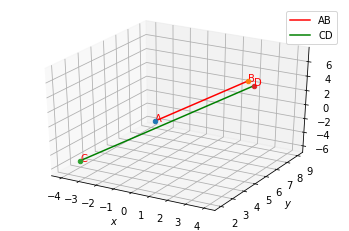
\includegraphics[width=\columnwidth]{solutions/aug/2/32/figures/lines.png}
\caption{Plot of lines AB and CD}
\label{aug/2/ex/32fig:lines}
\end{figure}

